\section{Cadre de l'organisation}
\section{Statuts}
\section{Délégation de Service Public}
\section{Diagrammes de gestion}
\subsection{Organigramme}
\subsection{Diagramme de flux}
\subsection{Chaîne de fin de stock au Grand Café}

\begin{center}
\begin{dot2tex}
digraph FinStockBar {
  size = "7";
  rankdir = "LR";
  node [ shape = "circle", style = filled, fillcolor=lightgray ];
  SI [ shape = "octagon" ];
  F [ shape = "doublecircle" ];
  SI -> S [ label = "1" ] ;
  S -> R [ label = "2" ];
  R -> F [ label = "3" ];
  F -> S [ label = "4" ];
  S -> SI [ label = "5" ];
  S -> C [ label = "6" ];
  C -> SI [ label = "7" ];
  C -> F [ label = "8" ];
  C -> SI [ label = "9" ];
}
\include{
\end{dot2tex}
\end{center}
\begin{enumerate}
\item Le SI (caisse du Grand Café) indique au S (serveur) une fin de stock ;
\item Le S transmet l'information au responsable stocks (R) ;
\item Le R passe une commande au fournisseur (F) ;
\item F livre le produit, fournit un bon de livraison et une facture au S ;
\item Le S met à jour le stock dans le SI ;
\item Le S transmet le bon de livraison et la facture au comptable (C) ;
\item Le S saisit la facture dans le SI ;
\item Le S effectue le règlement (8) auprès du F ;
\item Le S l'indique au SI.
\end{enumerate}

\subsection{Exemples de commandes}
\pagebreak
\section{Illustration des outils}
\subsection{Gestion des incidents}
\label{gestion_incidents}
\begin{figure}[!h]
	\centering
	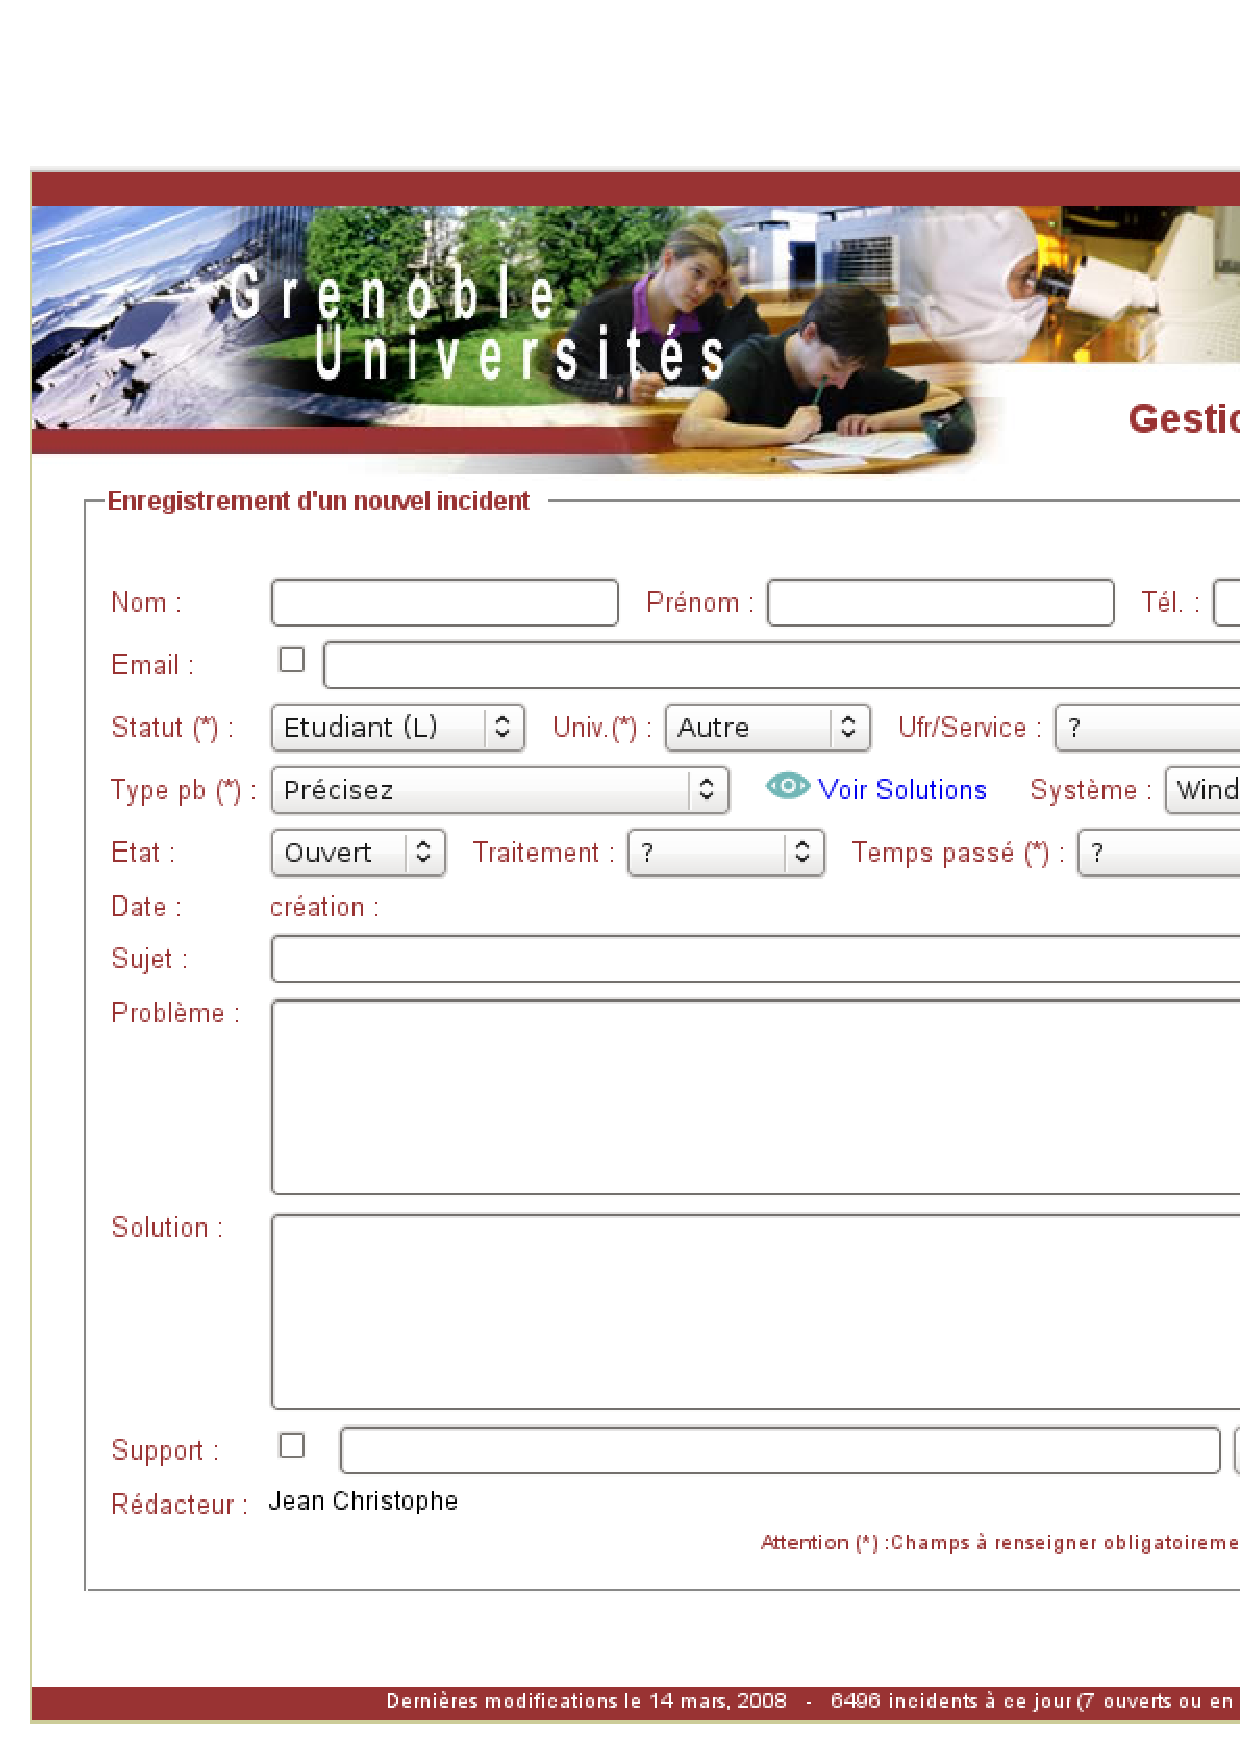
\includegraphics[width=12cm]{annexes/gestion_des_incidents.png}
	\caption{Interface de saisie de l'application de gestion des incidents de l'assistance informatique.}
\end{figure}
\clearpage
\section{Modèles et exemples de pièces}
\subsection{A}

